\chapter{Matrix}
\section{LC 0200 - Number of Islands}
Given an {\colorbox{CodeBackground}{\lstinline|m x n|}} binary grid {\colorbox{CodeBackground}{\lstinline|grid|}} which represents a map of {\colorbox{CodeBackground}{\lstinline|'1'|}}s (\ul{land}) and {\colorbox{CodeBackground}{\lstinline|'0'|}}s (\ul{water}), return the number of \ul{islands}.\\

An \ul{island} is surrounded by water and is formed by connecting adjacent lands horizontally or vertically. \\

You may assume all four edges of {\colorbox{CodeBackground}{\lstinline|grid|}} are all surrounded by water.\\

\begin{itemize}
\item Example 1
\begin{lstlisting}
[["1","1","1","1","0"],
 ["1","1","0","1","0"],
 ["1","1","0","0","0"],
 ["0","0","0","0","0"]] --> 1
\end{lstlisting}
\item Example 2
\begin{lstlisting}
[["1","1","0","0","0"],
 ["1","1","0","0","0"],
 ["0","0","1","0","0"],
 ["0","0","0","1","1"]] --> 3
\end{lstlisting}
\end{itemize}

\subsection*{Solution 1 - DFS}
\begin{lstlisting}
int numIslands(std::vector<std::vector<char>>& grid) {
  int num_island = 0;
  for (int i = 0; i < grid.size(); ++i) {
    for (int j = 0; j < grid[0].size(); ++j) {
      if (grid[i][j] == '1') {
        DFSSinkLand(grid, i, j);
        ++num_island;
      }
    }
  }
  return num_island;
}

void DFSSinkLand(std::vector<std::vector<char>>& grid, int i, int j) {
  if (i < 0 || i >= grid.size() || j < 0 || j >= grid[0].size()) { return; }
  if (grid[i][j] == '0') { return; }
  grid[i][j] = '0';
  DFSSinkLand(grid, i - 1, j);
  DFSSinkLand(grid, i + 1, j);
  DFSSinkLand(grid, i, j - 1);
  DFSSinkLand(grid, i, j + 1);
}
\end{lstlisting}

\subsection*{Solution 2 - BFS}
\begin{lstlisting}
int numIslands(std::vector<std::vector<char>>& grid) {
  if (grid.empty()) { return 0; }
  int num_island = 0;
  for (int i = 0; i < grid.size(); ++i) {
    for (int j = 0; j < grid[0].size(); ++j) {
      if (grid[i][j] == '1') {
        BFS(grid, i, j);
        ++num_island;
      }
    }
  }
  return num_island;
}

void BFS(std::vector<std::vector<char>>& grid, int i, int j) {
  std::queue<std::pair<int, int>> q;
  q.emplace(i, j);
  grid[i][j] = '0';
  std::vector<std::pair<int, int>> dirs = {{-1, 0}, {1, 0}, {0, -1}, {0, 1}};
  while (!q.empty()) {
    auto [r, c] = q.front();
    q.pop();
    for (auto [dr, dc] : dirs) {
      int new_r = r + dr;
      int new_c = c + dc;
      if (new_r >= 0 && new_r < grid.size() && new_c >= 0 && new_c < grid[0].size()
          && grid[new_r][new_c] == '1') {
        q.emplace(new_r, new_c);
        grid[new_r][new_c] = '0';
      }
    }
  }
}
\end{lstlisting}

\subsection*{Solution 3 - BFS (Time Limit Exceeded)}
The only difference between Solution 2 and Solution 3 lies in the timing of sinking a land cell.
\begin{itemize}
\item Solution 2 sinks the neighboring land cells before enqueuing them.
\item Solution 3 delays this sinking until after the land cell is dequeued.
\end{itemize}

This state of cells influences whether or not BFS decides to explore the neighboring cells. A smart choice it to update those states as early as we can. If we wait too long to sink lands, we might end up enqueuing duplicate land cells again and again, which, in the best-case scenario, reduces the algorithm's speed and, in the worst-case scenario, leads to an infinite loop.\\

See the more general form of this issue here: \hyperref[subsubsec:graph_universal_implementation_bfs]{Graph (Universal Implementation) - BFS}.

\begin{lstlisting}
int numIslands(std::vector<std::vector<char>>& grid) {
  if (grid.empty()) { return 0; }
  int num_island = 0;
  for (int i = 0; i < grid.size(); ++i) {
    for (int j = 0; j < grid[0].size(); ++j) {
      if (grid[i][j] == '1') {
        BFSSinkLand(grid, i, j);
        ++num_island;
      }
    }
  }
  return num_island;
}

void BFSSinkLand(std::vector<std::vector<char>>& grid, int i, int j) {
  std::queue<std::pair<int, int>> q;
  q.emplace(i, j);
  grid[i][j] = '0';
  std::vector<std::pair<int, int>> dirs = {{-1, 0}, {1, 0}, {0, -1}, {0, 1}};
  while (!q.empty()) {
    auto [r, c] = q.front();
    q.pop();
    grid[r][c] = '0';
    for (auto [dr, dc] : dirs) {
      int new_r = r + dr;
      int new_c = c + dc;
      if (new_r >= 0 && new_r < grid.size() && new_c >= 0 && new_c < grid[0].size()
          && grid[new_r][new_c] == '1') {
        q.emplace(new_r, new_c);
      }
    }
  }
}
\end{lstlisting}

\section{LC 1020 - Number of Enclaves}
You are given an {\colorbox{CodeBackground}{\lstinline|m x n|}} binary matrix {\colorbox{CodeBackground}{\lstinline|grid|}}, where {\colorbox{CodeBackground}{\lstinline|0|}} represents a \ul{sea cell} and {\colorbox{CodeBackground}{\lstinline|1|}} represents a \ul{land cell}.\\

A \ul{move} consists of:
\begin{itemize}
\item walking from one \ul{land cell} to another adjacent ({\colorbox{CodeBackground}{\lstinline|4|}}-directionally) \ul{land cell}
\item or walking off the boundary of the {\colorbox{CodeBackground}{\lstinline|grid|}}.
\end{itemize}

Return the number of \ul{land cells} in {\colorbox{CodeBackground}{\lstinline|grid|}} for which we cannot walk off the boundary of the {\colorbox{CodeBackground}{\lstinline|grid|}} in any number of moves.\\

\begin{itemize}
	\item Example 1
\begin{lstlisting}
[[0,0,0,0],
 [1,0,1,0],
 [0,1,1,0],
 [0,0,0,0]] --> 3
\end{lstlisting}
	\begin{figure}[H]
		\centering
		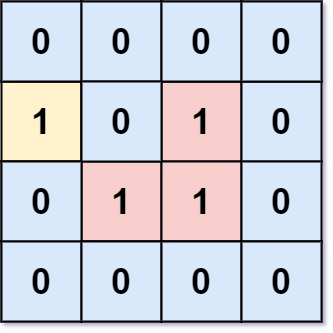
\includegraphics[width=0.2\linewidth]{images/lc1020_eg1}
		\label{fig:lc1020eg1}
	\end{figure}
	\item Example 2
\begin{lstlisting}
[[0,1,1,0],
 [0,0,1,0],
 [0,0,1,0],
 [0,0,0,0]] --> 0
\end{lstlisting}
	\begin{figure}[H]
		\centering
		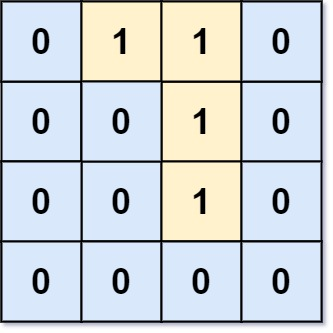
\includegraphics[width=0.2\linewidth]{images/lc1020_eg2}
		\label{fig:lc1020eg2}
	\end{figure}
\end{itemize}

\subsection*{Solution 1 - DFS}
\begin{lstlisting}
int numEnclaves(std::vector<std::vector<int>>& grid) {
  int m = grid.size();
  int n = grid[0].size();
  for (int i = 0; i < m; ++i) {
    DFSSinkLand(grid, i, 0);
    DFSSinkLand(grid, i, n - 1);
  }
  for (int j = 1; j < n - 1; ++j) {
    DFSSinkLand(grid, 0, j);
    DFSSinkLand(grid, m - 1, j);
  }
  int count = 0;
  for (int i = 1; i < m - 1; ++i) {
    for (int j = 1; j < n - 1; ++j) {
      if (grid[i][j] == 1) { ++count; }
    }
  }
  return count;
}

void DFSSinkLand(std::vector<std::vector<int>>& grid, int i, int j) {
  if (i < 0 || i >= grid.size() || j < 0 || j >= grid[0].size()) { return; }
  if (grid[i][j] == 0) { return; }
  grid[i][j] = 0;
  DFSSinkLand(grid, i - 1, j);
  DFSSinkLand(grid, i + 1, j);
  DFSSinkLand(grid, i, j - 1);
  DFSSinkLand(grid, i, j + 1);
}
\end{lstlisting}

\subsection*{Solution 2 - BFS}
\begin{lstlisting}
int numEnclaves(std::vector<std::vector<int>>& grid) {
  int m = grid.size();
  int n = grid[0].size();
  std::queue<std::pair<int, int>> q;
  for (int i = 0; i < m; ++i) {
    if (grid[i][0] == 1) { q.emplace(i, 0); }
    if (grid[i][n - 1] == 1) { q.emplace(i, n - 1); }
  }
  for (int j = 1; j < n - 1; ++j) {
    if (grid[0][j] == 1) { q.emplace(0, j); }
    if (grid[m - 1][j] == 1) { q.emplace(m - 1, j); }
  }
  std::vector<std::pair<int, int>> dirs = {{-1, 0}, {1, 0}, {0, -1}, {0, 1}};
  while (!q.empty()) {
    auto [r, c] = q.front();
    q.pop();
    for (auto [dr, dy] : dirs) {
      int new_r = r + dr;
      int new_c = c + dy;
      if (new_r >= 0 && new_r < m && new_c >= 0 && new_c < n && grid[new_r][new_c] == 1) {
        q.emplace(new_r, new_c);
        grid[new_r][new_c] = 0;
      }
    }
  }
  int count = 0;
  for (int i = 1; i < m - 1; ++i) {
    for (int j = 1; j < n - 1; ++j) {
      if (grid[i][j] == 1) { ++count; }
    }
  }
  return count;
}
\end{lstlisting}

\section{LC 0463 - Island Perimeter}
You are given {\colorbox{CodeBackground}{\lstinline|m x n|}} {\colorbox{CodeBackground}{\lstinline|grid|}} representing a map where {\colorbox{CodeBackground}{\lstinline|1|}} represents \ul{land} and {\colorbox{CodeBackground}{\lstinline|0|}} represents \ul{water}.\\

An \ul{island} is a group of {\colorbox{CodeBackground}{\lstinline|1|}}'s (representing land) connected {\colorbox{CodeBackground}{\lstinline|4|}}-directionally (horizontal or vertical). \\

You may assume all four edges of the {\colorbox{CodeBackground}{\lstinline|grid|}} are surrounded by water.\\

In this question, the island doesn't have "lakes", meaning the water inside isn't connected to the water around the island. And there is exactly one island in {\colorbox{CodeBackground}{\lstinline|grid|}}.\\

Determine the perimeter of the island.

\begin{itemize}
\item Example 1
\begin{lstlisting}
[[0,1,0,0],
 [1,1,1,0],
 [0,1,0,0],
 [1,1,0,0]] --> 16
\end{lstlisting}
\begin{figure}[H]
\centering
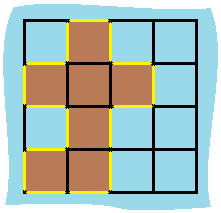
\includegraphics[width=0.2\linewidth]{images/lc0463_eg}
\label{fig:lc0463eg}
\end{figure}
\item Example 2
\begin{lstlisting}
grid = [[1]] --> 4
\end{lstlisting}
\item Example 3
\begin{lstlisting}
grid = [[1,0]] --> 4
\end{lstlisting}
\end{itemize}

\subsection*{Solution 1 - Brute Force}
\begin{lstlisting}
int islandPerimeter(std::vector<std::vector<int>>& grid) {
  int perimeter = 0;
  for (int i = 0; i < grid.size(); ++i) {
    for (int j = 0; j < grid[0].size(); ++j) {
      if (grid[i][j] == 1) {
        if (i == 0 || grid[i - 1][j] == 0) { perimeter++; }
        if (i == grid.size() - 1 || grid[i + 1][j] == 0) { perimeter++; }
        if (j == 0 || grid[i][j - 1] == 0) { perimeter++; }
        if (j == grid[0].size() - 1 || grid[i][j + 1] == 0) { perimeter++; }
      }
    }
  }
  return perimeter;
}
\end{lstlisting}

\subsection*{Solution 2 - Count Lands and Connections}
\begin{lstlisting}
int islandPerimeter(std::vector<std::vector<int>>& grid) {
  int num_lands = 0;
  int num_connections = 0;
  int m = grid.size();
  int n = grid[0].size();
  for (int i = 0; i < m; ++i) {
    for (int j = 0; j < n; ++j) {
      if (grid[i][j] == 1) {
        ++num_lands;
        if (j < n - 1 && grid[i][j + 1] == 1) { ++num_connections; }
        if (i < m - 1 && grid[i + 1][j] == 1) { ++num_connections; }
      }
    }
  }
  return 4 * num_lands - 2 * num_connections;
}
\end{lstlisting}

\section{LC 0130 - Surrounded Regions}
Given an {\colorbox{CodeBackground}{\lstinline|m x n|}} matrix {\colorbox{CodeBackground}{\lstinline|board|}} containing {\colorbox{CodeBackground}{\lstinline|'X'|}} and {\colorbox{CodeBackground}{\lstinline|'O'|}}, \ul{capture} all regions that are {\colorbox{CodeBackground}{\lstinline|4|}}-directionally surrounded by {\colorbox{CodeBackground}{\lstinline|'X'|}}. \\

A region is \ul{captured} by flipping all {\colorbox{CodeBackground}{\lstinline|'O'|}}s into {\colorbox{CodeBackground}{\lstinline|'X'|}}s in that surrounded region.

\begin{itemize}
\item Example 1
\begin{lstlisting}
[["X","X","X","X"],
 ["X","O","O","X"],
 ["X","X","O","X"],
 ["X","O","X","X"]]
--> 
[["X","X","X","X"],
 ["X","X","X","X"],
 ["X","X","X","X"],
 ["X","O","X","X"]]

\end{lstlisting}
\begin{figure}[H]
\centering
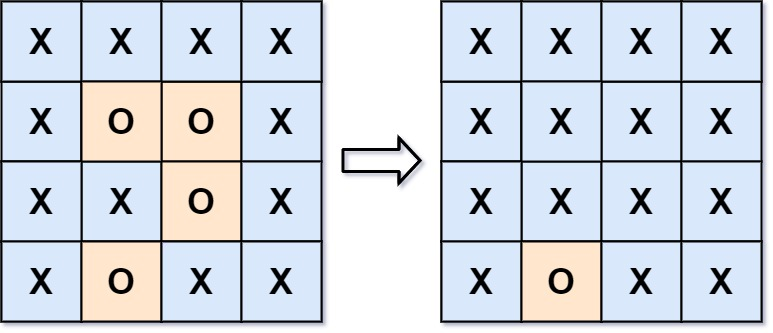
\includegraphics[width=0.4\linewidth]{images/lc0130_eg}
\label{fig:lc0130eg}
\end{figure}
\item Example 2
\begin{lstlisting}
[["X"]] --> [["X"]]
\end{lstlisting}
\end{itemize}

\subsection*{Solution - DFS}
\begin{lstlisting}
void solve(std::vector<std::vector<char>>& board) {
  int m = board.size();
  int n = board[0].size();
  // mark 'O's on border and connected to border as 'S' (safe)
  for (int i = 0; i < m; ++i) {
    if (board[i][0] == 'O') { DFSMarkSafe(board, i, 0); }
    if (board[i][n - 1] == 'O') { DFSMarkSafe(board, i, n - 1); }
  }
  for (int j = 0; j < n; ++j) {
    if (board[0][j] == 'O') { DFSMarkSafe(board, 0, j); }
    if (board[m - 1][j] == 'O') { DFSMarkSafe(board, m - 1, j); }
  }
  // flip 'O's to 'X's and 'S's back to 'O's
  for (int i = 0; i < m; ++i) {
    for (int j = 0; j < n; ++j) {
      if (board[i][j] == 'O') { board[i][j] = 'X'; }
      if (board[i][j] == 'S') { board[i][j] = 'O'; }
    }
  }
}

void DFSMarkSafe(std::vector<std::vector<char>>& board, int i, int j) {
  if (i < 0 || i >= board.size() || j < 0 || j >= board[0].size()) { return; }
  if (board[i][j] != 'O') { return; }
  board[i][j] = 'S';
  DFSMarkSafe(board, i - 1, j);
  DFSMarkSafe(board, i + 1, j);
  DFSMarkSafe(board, i, j - 1);
  DFSMarkSafe(board, i, j + 1);
}
\end{lstlisting}

\section{LC 0733 - Flood Fill}
An image is represented by an {\colorbox{CodeBackground}{\lstinline|m x n|}} integer grid {\colorbox{CodeBackground}{\lstinline|image|}} where {\colorbox{CodeBackground}{\lstinline|image[i][j]|}} represents the pixel value of the image.\\

You are also given three integers {\colorbox{CodeBackground}{\lstinline|sr|}}, {\colorbox{CodeBackground}{\lstinline|sc|}}, and {\colorbox{CodeBackground}{\lstinline|color|}}. You should perform a \ul{flood fill} on the image starting from the pixel {\colorbox{CodeBackground}{\lstinline|image[sr][sc]|}}.\\

To perform a \ul{flood fill}, consider:
\begin{enumerate}
\item the starting pixel;
\item plus any pixels connected {\colorbox{CodeBackground}{\lstinline|4|}}-directionally to the starting pixel of the same color as the starting pixel;
\item plus any pixels connected {\colorbox{CodeBackground}{\lstinline|4|}}-directionally to those pixels (also with the same color);
\item and so on.
\end{enumerate}
Replace the color of all of the aforementioned pixels with {\colorbox{CodeBackground}{\lstinline|color|}}.\\

Return the modified image after performing the \ul{flood fill}.\\

\begin{itemize}
\item Example 1
\begin{lstlisting}
image = 
[[1,1,1],
 [1,1,0],
 [1,0,1]]
sr = 1, sc = 1, color = 2
--> 
[[2,2,2],
 [2,2,0],
 [2,0,1]]
\end{lstlisting}
\begin{figure}[H]
\centering
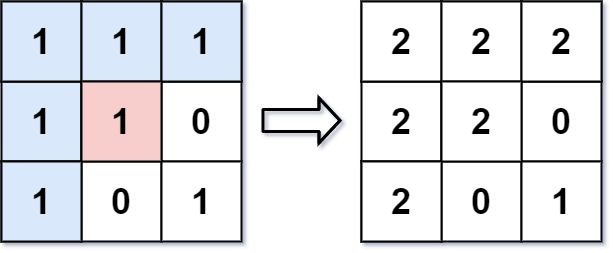
\includegraphics[width=0.4\linewidth]{images/lc0733_eg}
\label{fig:lc0733eg}
\end{figure}
\item Example 2
\begin{lstlisting}
image = 
[[0,0,0],
 [0,0,0]]
sr = 0, sc = 0, color = 0
-->
[[0,0,0],
 [0,0,0]]
\end{lstlisting}
\end{itemize}

\subsection*{Solution - DFS}
\begin{lstlisting}
void dfs(std::vector<std::vector<int>>& image, int sr, int sc, int newColor, int oldColor) {
	if (sr < 0 || sc < 0 || sr >= image.size() || sc >= image[0].size()
	|| image[sr][sc] != oldColor) {
		return;
	}
	
	image[sr][sc] = newColor;
	
	// Flood fill in all 4 directions
	dfs(image, sr + 1, sc, newColor, oldColor);
	dfs(image, sr - 1, sc, newColor, oldColor);
	dfs(image, sr, sc + 1, newColor, oldColor);
	dfs(image, sr, sc - 1, newColor, oldColor);
}

std::vector<std::vector<int>> floodFill(std::vector<std::vector<int>>& image, int sr, int sc,
int newColor) {
	int oldColor = image[sr][sc];
	if (oldColor
	!= newColor) {  // Only fill if the new color is different to avoid infinite recursion
		dfs(image, sr, sc, newColor, oldColor);
	}
	return image;
}
\end{lstlisting}

\section{LC 0994 - Rotting Oranges}
You are given an {\colorbox{CodeBackground}{\lstinline|m x n|}} grid where each cell can have one of three values:
\begin{itemize}
\item {\colorbox{CodeBackground}{\lstinline|0|}} representing an \ul{empty cell};
\item {\colorbox{CodeBackground}{\lstinline|1|}} representing a \ul{fresh orange};
\item {\colorbox{CodeBackground}{\lstinline|2|}} representing a \ul{rotten orange};
\end{itemize}

Every minute, any fresh orange that is {\colorbox{CodeBackground}{\lstinline|4|}}-directionally adjacent to a rotten orange becomes rotten.\\

Return the minimum number of minutes that must elapse until no cell has a fresh orange. If this is impossible, return {\colorbox{CodeBackground}{\lstinline|-1|}}.

\begin{itemize}
\item Example 1
\begin{lstlisting}
[[2,1,1],
[1,1,0],
[0,1,1]] --> 4
\end{lstlisting}
\begin{figure}[H]
\centering
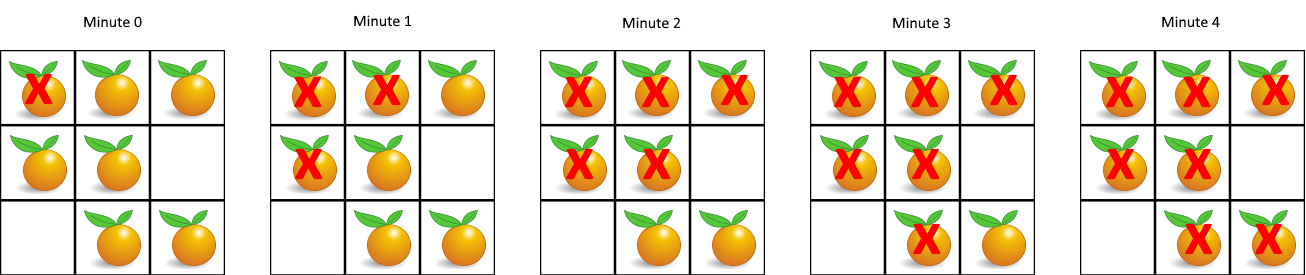
\includegraphics[width=0.8\linewidth]{images/lc0994_example}
\label{fig:lc0994example}
\end{figure}
\item Example 2
\begin{lstlisting}
[[2,1,1],
 [0,1,1],
 [1,0,1]] --> -1
\end{lstlisting}
\item Example 3
\begin{lstlisting}
[[0,2]] --> 0
\end{lstlisting}
\end{itemize}

\subsection*{Solution - BFS + Record Level}
\begin{lstlisting}
int orangesRotting(std::vector<std::vector<int>>& grid) {
  int m = grid.size();
  int n = grid[0].size();
  std::queue<std::pair<int, int>> q;
  int num_fresh = 0;
  for (int i = 0; i < m; ++i) {
    for (int j = 0; j < n; ++j) {
      if (grid[i][j] == 2) { q.emplace(i, j); }
      if (grid[i][j] == 1) { ++num_fresh; }
    }
  }
  int level = 0;
  std::vector<std::pair<int, int>> dirs = {{-1, 0}, {1, 0}, {0, -1}, {0, 1}};
  while (!q.empty() && num_fresh > 0) {
    ++level;
    int level_size = q.size();
    for (int i = 0; i < level_size; ++i) {
      auto [r, c] = q.front();
      q.pop();
      for (auto [dr, dc] : dirs) {
        int new_r = r + dr;
        int new_c = c + dc;
        if (new_r >= 0 && new_c >= 0 && new_r < m && new_c < n && grid[new_r][new_c] == 1) {
          grid[new_r][new_c] = 2;
          --num_fresh;
          q.emplace(new_r, new_c);
        }
      }
    }
  }
  if (num_fresh > 0) { return -1; }
  return level;
}
\end{lstlisting}

\section{LC 1197 - Minimum Knight Moves}
In an \ul{infinite chess board} with coordinates from {\colorbox{CodeBackground}{\lstinline|-inf|}} to {\colorbox{CodeBackground}{\lstinline|+inf|}}. \\

A knight has \ul{{\colorbox{CodeBackground}{\lstinline|8|}} possible moves} it can make, as illustrated below. Each move is two squares in a \ul{cardinal direction}, then one square in an \ul{orthogonal direction}.

\begin{figure}[H]
\centering
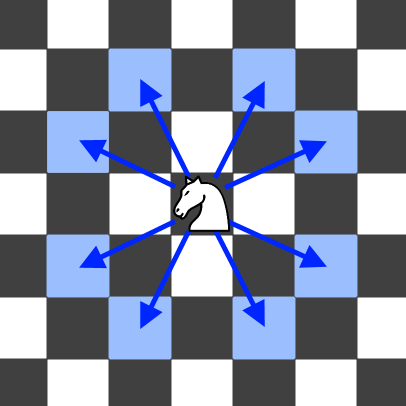
\includegraphics[width=0.25\linewidth]{images/lc1197}
\label{fig:lc1197}
\end{figure}

Return the minimum number of steps needed to move the knight from square {\colorbox{CodeBackground}{\lstinline|[0, 0]|}} to square {\colorbox{CodeBackground}{\lstinline|[x, y]|}}. It is guaranteed the answer exists.\\

Examples:
\begin{itemize}
\item {\colorbox{CodeBackground}{\lstinline|x = 2, y = 1 --> 1|}}
\item {\colorbox{CodeBackground}{\lstinline|x = 5, y = 5 --> 4|}}
\end{itemize}

\subsection*{*Solution - BFS (Time Limit Exceeded)}
\begin{lstlisting}
int minKnightMoves(int x, int y) {
	std::vector<std::vector<int>> moves = {{1, 2}, {1, -2}, {-1, 2}, {-1, -2},
																				 {2, 1}, {2, -1}, {-2, 1}, {-2, -1}};
	std::set<std::pair<int, int>> visited;
	std::queue<std::pair<std::pair<int, int>, int>> q;
	q.push({{0, 0}, 0});
	visited.insert({0, 0});
	while (!q.empty()) {
		auto& front = q.front();
		auto cur_pos = front.first;
		int num_move = front.second;
		q.pop();
		if (cur_pos.first == x && cur_pos.second == y) { return num_move; }
		for (const auto& move : moves) {
			int next_x = cur_pos.first + move[0];
			int next_y = cur_pos.second + move[1];
			std::pair<int, int> next_pos = {next_x, next_y};
			if (visited.find(next_pos) == visited.end()) {
				q.push({next_pos, num_move + 1});
				visited.insert(next_pos);
			}
		}
	}
	return -1;
}
\end{lstlisting}

\section{LC 0417 - Pacific Atlantic Water Flow}
There is an {\colorbox{CodeBackground}{\lstinline|m x n|}} rectangular island that borders both the \ul{Pacific Ocean} and \ul{Atlantic Ocean}. The \ul{Pacific Ocean} touches the island's \ul{left and top edges}, and the \ul{Atlantic Ocean} touches the island's \ul{right and bottom edges}.\\

The island is partitioned into a grid of square cells. You are given an {\colorbox{CodeBackground}{\lstinline|m x n|}} integer matrix {\colorbox{CodeBackground}{\lstinline|heights|}} where {\colorbox{CodeBackground}{\lstinline|heights[r][c]|}} represents \ul{the height above sea level} of the cell at coordinate {\colorbox{CodeBackground}{\lstinline|(r, c)|}}.\\

The island receives a lot of rain, and the rain water can flow to neighboring cells directly north, south, east, and west if the neighboring cell's height is less than or equal to the current cell's height. Water can flow from any cell adjacent to an ocean into the ocean.\\

Return a 2D list of grid coordinates {\colorbox{CodeBackground}{\lstinline|result|}} where {\colorbox{CodeBackground}{\lstinline|result[i] = [r_i, c_i]|}} denotes that rain water can flow from cell {\colorbox{CodeBackground}{\lstinline|(r_i, c_i)|}} to both the Pacific and Atlantic oceans.\\

\begin{itemize}
\item Example 1
\begin{lstlisting}
heights = 
[[1,2,2,3,5],
 [3,2,3,4,4],
 [2,4,5,3,1],
 [6,7,1,4,5],
 [5,1,1,2,4]]
--> [[0,4],[1,3],[1,4],[2,2],[3,0],[3,1],[4,0]]
\end{lstlisting}
\begin{figure}[H]
\centering
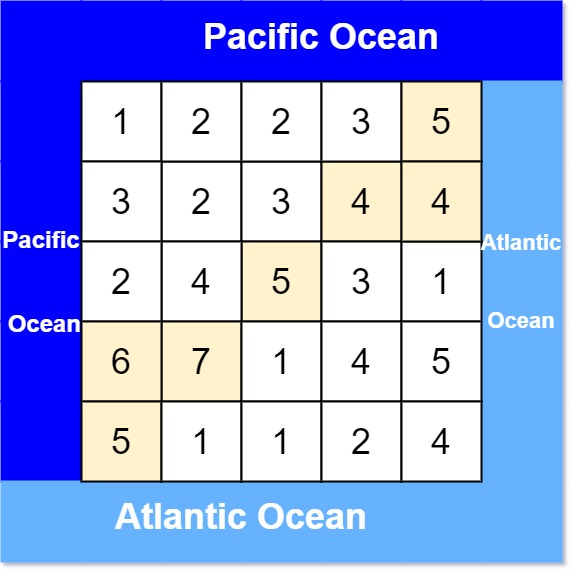
\includegraphics[width=0.3\linewidth]{images/lc0417_eg}
\label{fig:lc0417eg}
\end{figure}
\item Example 2
\begin{lstlisting}
heights = [[1]] --> [[0,0]]
\end{lstlisting}
\end{itemize}


\subsection*{Solution - DFS}
\begin{lstlisting}
void DFS(const std::vector<std::vector<int>>& heights, std::vector<std::vector<bool>>& can_reach,
int r, int c) {
	if (can_reach[r][c]) { return; }
	can_reach[r][c] = true;
	std::vector<std::pair<int, int>> dirs = {{0, 1}, {1, 0}, {-1, 0}, {0, -1}};
	for (auto& dir : dirs) {
		int new_r = r + dir.first, new_c = c + dir.second;
		if (new_r >= 0 && new_r < heights.size() && new_c >= 0 && new_c < heights[0].size()
		&& heights[new_r][new_c] >= heights[r][c]) {
			DFS(heights, can_reach, new_r, new_c);
		}
	}
}

std::vector<std::vector<int>> pacificAtlantic(std::vector<std::vector<int>>& heights) {
	if (heights.empty()) return {};
	
	int m = heights.size();
	int n = heights[0].size();
	std::vector<std::vector<bool>> canReachP(m, std::vector<bool>(n, false));
	std::vector<std::vector<bool>> canReachA(m, std::vector<bool>(n, false));
	std::vector<std::vector<int>> result;
	
	for (int i = 0; i < m; ++i) {
		DFS(heights, canReachP, i, 0);      // Pacific left border
		DFS(heights, canReachA, i, n - 1);  // Atlantic right border
	}
	
	for (int i = 0; i < n; ++i) {
		DFS(heights, canReachP, 0, i);      // Pacific top border
		DFS(heights, canReachA, m - 1, i);  // Atlantic bottom border
	}
	
	for (int r = 0; r < m; ++r) {
		for (int c = 0; c < n; ++c) {
			if (canReachP[r][c] && canReachA[r][c]) { result.push_back({r, c}); }
		}
	}
	
	return result;
}
\end{lstlisting}

\section{LC 0695 - Max Area of Island}
Given an {\colorbox{CodeBackground}{\lstinline|m x n|}} binary matrix {\colorbox{CodeBackground}{\lstinline|grid|}}, return the maximum area of an \ul{island} in {\colorbox{CodeBackground}{\lstinline|grid|}}. If there is no island, return {\colorbox{CodeBackground}{\lstinline|0|}}.\\


An \ul{island} is a group of {\colorbox{CodeBackground}{\lstinline|1|}}'s (representing land) connected {\colorbox{CodeBackground}{\lstinline|4|}}-directionally (horizontal or vertical.) \\

You may assume all four edges of the {\colorbox{CodeBackground}{\lstinline|grid|}} are surrounded by water.

\begin{itemize}
\item Example 1
\begin{lstlisting}
[[0,0,1,0,0,0,0,1,0,0,0,0,0],
 [0,0,0,0,0,0,0,1,1,1,0,0,0],
 [0,1,1,0,1,0,0,0,0,0,0,0,0],
 [0,1,0,0,1,1,0,0,1,0,1,0,0],
 [0,1,0,0,1,1,0,0,1,1,1,0,0],
 [0,0,0,0,0,0,0,0,0,0,1,0,0],
 [0,0,0,0,0,0,0,1,1,1,0,0,0],
 [0,0,0,0,0,0,0,1,1,0,0,0,0]] --> 6
\end{lstlisting}
\begin{figure}[H]
\centering
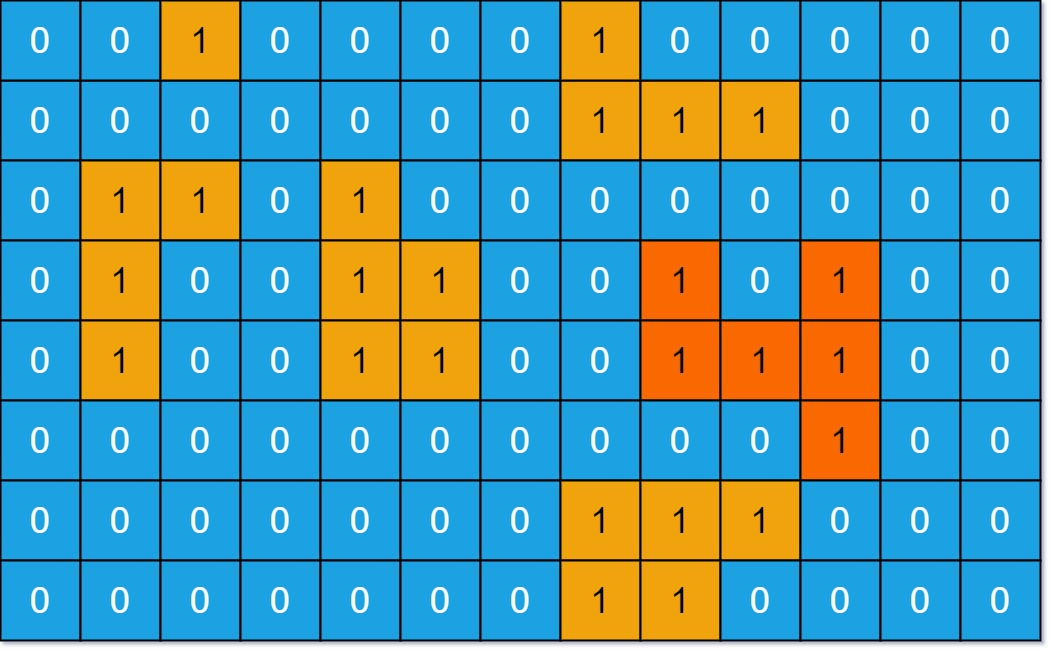
\includegraphics[width=0.6\linewidth]{images/lc0695_example}
\label{fig:lc0695example}
\end{figure}
\item Example 2
\begin{lstlisting}
[[0,0,0,0,0,0,0,0]] --> 0
\end{lstlisting}
\end{itemize}

\subsection*{Solution 1 - DFS}
\begin{lstlisting}
int maxAreaOfIsland(std::vector<std::vector<int>>& grid) {
  int max_area = 0;
  for (int i = 0; i < grid.size(); ++i) {
    for (int j = 0; j < grid[0].size(); ++j) {
      if (grid[i][j] == 1) {
        int area = 0;
        DFSSinkLandAndIncreaseArea(grid, i, j, area);
        max_area = std::max(max_area, area);
      }
    }
  }
  return max_area;
}

void DFSSinkLandAndIncreaseArea(std::vector<std::vector<int>>& grid, int i, int j,
                                int& area) {
  if (i < 0 || i >= grid.size() || j < 0 || j >= grid[0].size()) { return; }
  if (grid[i][j] != 1) { return; }
  grid[i][j] = 0;
  area += 1;
  DFSSinkLandAndIncreaseArea(grid, i - 1, j, area);
  DFSSinkLandAndIncreaseArea(grid, i + 1, j, area);
  DFSSinkLandAndIncreaseArea(grid, i, j - 1, area);
  DFSSinkLandAndIncreaseArea(grid, i, j + 1, area);
}
\end{lstlisting}

\subsection*{Solution 2 - DFS with Return Value}
\begin{lstlisting}
int maxAreaOfIsland(std::vector<std::vector<int>>& grid) {
  int max_area = 0;
  for (int i = 0; i < grid.size(); ++i) {
    for (int j = 0; j < grid[0].size(); ++j) {
      if (grid[i][j] == 1) {
        max_area = std::max(max_area, DFSSinkLandAndCalcArea(grid, i, j));
      }
    }
  }
  return max_area;
}

int DFSSinkLandAndCalcArea(std::vector<std::vector<int>>& grid, int i, int j) {
  if (i < 0 || i >= grid.size() || j < 0 || j >= grid[0].size()) { return 0; }
  if (grid[i][j] != 1) { return 0; }
  grid[i][j] = 0;
  int area = 1;
  area += DFSSinkLandAndCalcArea(grid, i - 1, j);
  area += DFSSinkLandAndCalcArea(grid, i + 1, j);
  area += DFSSinkLandAndCalcArea(grid, i, j - 1);
  area += DFSSinkLandAndCalcArea(grid, i, j + 1);
  return area;
}
\end{lstlisting}

\section{LC 1905 - Count Sub Islands}
You are given two {\colorbox{CodeBackground}{\lstinline|m x n|}} binary matrices {\colorbox{CodeBackground}{\lstinline|grid1|}} and {\colorbox{CodeBackground}{\lstinline|grid2|}} containing only {\colorbox{CodeBackground}{\lstinline|0|}}'s (representing \ul{water}) and {\colorbox{CodeBackground}{\lstinline|1|}}'s (representing \ul{land}). Any cells outside of the grid are considered water cells.\\

An island is a group of {\colorbox{CodeBackground}{\lstinline|1|}}'s connected {\colorbox{CodeBackground}{\lstinline|4|}}-directionally (horizontal or vertical).\\

An island in {\colorbox{CodeBackground}{\lstinline|grid2|}} is considered a \ul{sub-island} if there is an island in {\colorbox{CodeBackground}{\lstinline|grid1|}} that contains all the cells that make up this island in {\colorbox{CodeBackground}{\lstinline|grid2|}}.\\

Return the number of islands in {\colorbox{CodeBackground}{\lstinline|grid2|}} that are considered sub-islands.

\begin{itemize}
\item Example 1
\begin{lstlisting}
grad1 =
[[1,1,1,0,0],
 [0,1,1,1,1],
 [0,0,0,0,0],
 [1,0,0,0,0],
 [1,1,0,1,1]], 
grid2 = 
[[1,1,1,0,0],
 [0,0,1,1,1],
 [0,1,0,0,0],
 [1,0,1,1,0],
 [0,1,0,1,0]]
--> 3
\end{lstlisting}
\begin{figure}[H]
\centering
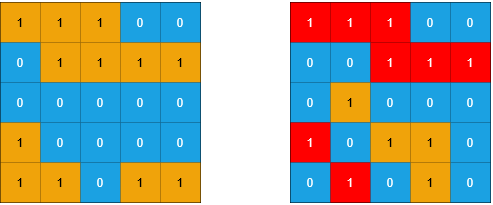
\includegraphics[width=0.6\linewidth]{images/lc1905_eg1}
\label{fig:lc1905eg1}
\end{figure}
\item Example 2
\begin{lstlisting}
grid1 = 
[[1,0,1,0,1],
 [1,1,1,1,1],
 [0,0,0,0,0],
 [1,1,1,1,1],
 [1,0,1,0,1]], 
grid2 = 
[[0,0,0,0,0],
 [1,1,1,1,1],
 [0,1,0,1,0],
 [0,1,0,1,0],
 [1,0,0,0,1]]
--> 2
\end{lstlisting}
\begin{figure}[H]
\centering
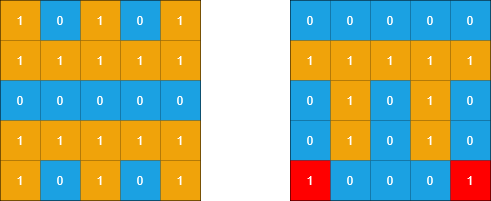
\includegraphics[width=0.6\linewidth]{images/lc1905_eg2}
\label{fig:lc1905eg2}
\end{figure}
\end{itemize}

\subsection*{Solution - DFS}
\begin{lstlisting}
int countSubIslands(std::vector<std::vector<int>>& grid1,
                    std::vector<std::vector<int>>& grid2) {
  int num_subislands = 0;
  for (int i = 0; i < grid2.size(); ++i) {
    for (int j = 0; j < grid2[0].size(); ++j) {
      if (grid2[i][j] == 1) {
        if (DFSCheckSubIsland(grid1, grid2, i, j)) { ++num_subislands; }
      }
    }
  }
  return num_subislands;
}

bool DFSCheckSubIsland(std::vector<std::vector<int>>& grid1,
                       std::vector<std::vector<int>>& grid2, int i, int j) {
  if (i < 0 || j < 0 || i >= grid2.size() || j >= grid2[0].size()) { return true; }
  if (grid2[i][j] == 0) { return true; }
  // doesn't meet the condition of a sub-island
  if (grid1[i][j] == 0) { return false; }
  // mark as visited
  grid2[i][j] = 0;
  bool up = DFSCheckSubIsland(grid1, grid2, i - 1, j);
  bool down = DFSCheckSubIsland(grid1, grid2, i + 1, j);
  bool left = DFSCheckSubIsland(grid1, grid2, i, j - 1);
  bool right = DFSCheckSubIsland(grid1, grid2, i, j + 1);
  return up && down && left && right;
}
\end{lstlisting}

\section{LC 0827 - Making A Large Island}
You are given an {\colorbox{CodeBackground}{\lstinline|n x n|}} binary matrix {\colorbox{CodeBackground}{\lstinline|grid|}} where {\colorbox{CodeBackground}{\lstinline|1|}} represents \ul{land} and {\colorbox{CodeBackground}{\lstinline|0|}} represents \ul{water}. \\

An island is a group of {\colorbox{CodeBackground}{\lstinline|1|}}'s connected {\colorbox{CodeBackground}{\lstinline|4|}}-directionally (horizontal or vertical).\\

You are allowed to change at \ul{most one} {\colorbox{CodeBackground}{\lstinline|0|}} to be {\colorbox{CodeBackground}{\lstinline|1|}}. \\

Return the size of the largest island in {\colorbox{CodeBackground}{\lstinline|grid|}} after applying this operation.

\begin{itemize}
\item Example 1
\begin{lstlisting}
[[1,0],
 [0,1]] --> 3
\end{lstlisting}
\item Example 2
\begin{lstlisting}
[[1,1],
 [1,0]] --> 4
\end{lstlisting}
\item Example 3
\begin{lstlisting}
[[1,1],
 [1,1]] --> 4
\end{lstlisting}
Can't change any {\colorbox{CodeBackground}{\lstinline|0|}} to {\colorbox{CodeBackground}{\lstinline|1|}}, only one island with {\colorbox{CodeBackground}{\lstinline|area = 4|}}.
\end{itemize}

\subsection*{Solution - DFS}
\begin{lstlisting}
int largestIsland(std::vector<std::vector<int>>& grid) {
  int max_size = 0;
  // 1. identify and mark islands and calculate their sizes
  std::unordered_map<int, int> id2size;
  int id = 2;
  for (int i = 0; i < grid.size(); ++i) {
    for (int j = 0; j < grid[i].size(); ++j) {
      if (grid[i][j] == 1) {
        int size = DFSMarkIslandAndCalcSize(grid, i, j, id);
        id2size[id++] = size;
        max_size = std::max(max_size, size);
      }
    }
  }
  // 2. flip each 0 to 1 to connect islands
  for (int i = 0; i < grid.size(); ++i) {
    for (int j = 0; j < grid[0].size(); ++j) {
      if (grid[i][j] == 0) {
        int new_size = 1;
        std::unordered_set<int> visited;
        std::vector<std::pair<int, int>> dirs = {{-1, 0}, {1, 0}, {0, -1}, {0, 1}};
        for (auto [dr, dc] : dirs) {
          int new_r = i + dr;
          int new_c = j + dc;
          if (new_r >= 0 && new_c >= 0 && new_r < grid.size() && new_c < grid[0].size()
              && grid[new_r][new_c] > 1) {
            int id = grid[new_r][new_c];
            if (visited.find(id) != visited.end()) { continue; }
            visited.insert(id);
            new_size += id2size[id];
          }
        }
        max_size = std::max(max_size, new_size);
      }
    }
  }
  return max_size;
}

int DFSMarkIslandAndCalcSize(std::vector<std::vector<int>>& grid, int i, int j, int id) {
  if (i < 0 || j < 0 || i >= grid.size() || j >= grid[0].size()) { return 0; }
  if (grid[i][j] != 1) { return 0; }
  grid[i][j] = id;
  int size = 1;
  size += DFSMarkIslandAndCalcSize(grid, i - 1, j, id);
  size += DFSMarkIslandAndCalcSize(grid, i + 1, j, id);
  size += DFSMarkIslandAndCalcSize(grid, i, j - 1, id);
  size += DFSMarkIslandAndCalcSize(grid, i, j + 1, id);
  return size;
}
\end{lstlisting}

\section{LC 0490 - The Maze}
There is a ball in a {\colorbox{CodeBackground}{\lstinline|maze|}} with \ul{empty spaces} (represented as {\colorbox{CodeBackground}{\lstinline|0|}}) and \ul{walls} (represented as {\colorbox{CodeBackground}{\lstinline|1|}}). You may assume that the borders of the maze are all walls (see examples). \\

The ball can go through the empty spaces by rolling \ul{up}, \ul{down}, \ul{left} or right, but it won't stop rolling until hitting a wall. When the ball stops, it could choose the next direction.\\

Given the {\colorbox{CodeBackground}{\lstinline|m x n|}} {\colorbox{CodeBackground}{\lstinline|maze|}}, the ball's {\colorbox{CodeBackground}{\lstinline|start|}} position and the {\colorbox{CodeBackground}{\lstinline|destination|}}, where {\colorbox{CodeBackground}{\lstinline|start = [start_row, start_col]|}} and {\colorbox{CodeBackground}{\lstinline|destination = [destination_row, destination_col]|}}, return {\colorbox{CodeBackground}{\lstinline|true|}} if the ball can stop at the destination, otherwise return {\colorbox{CodeBackground}{\lstinline|false|}}.

\begin{itemize}
\item Example 1
\begin{lstlisting}
maze = 
[[0,0,1,0,0],
 [0,0,0,0,0],
 [0,0,0,1,0],
 [1,1,0,1,1],
 [0,0,0,0,0]]
start = [0,4], destination = [4,4]
--> true
\end{lstlisting}
\begin{figure}[H]
\centering
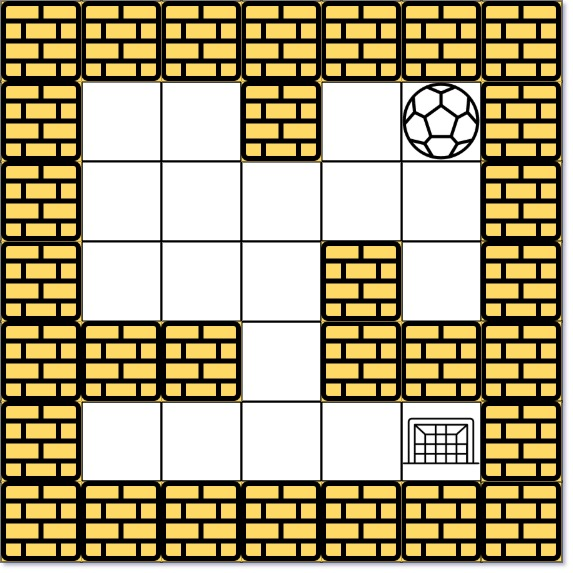
\includegraphics[width=0.25\linewidth]{images/lc0490_eg1}
\label{fig:lc0490eg1}
\end{figure}
\item Example 2
\begin{lstlisting}
maze = 
[[0,0,1,0,0],
 [0,0,0,0,0],
 [0,0,0,1,0],
 [1,1,0,1,1],
 [0,0,0,0,0]]
start = [0,4], destination = [3,2]
--> false
\end{lstlisting}
\begin{figure}[H]
\centering
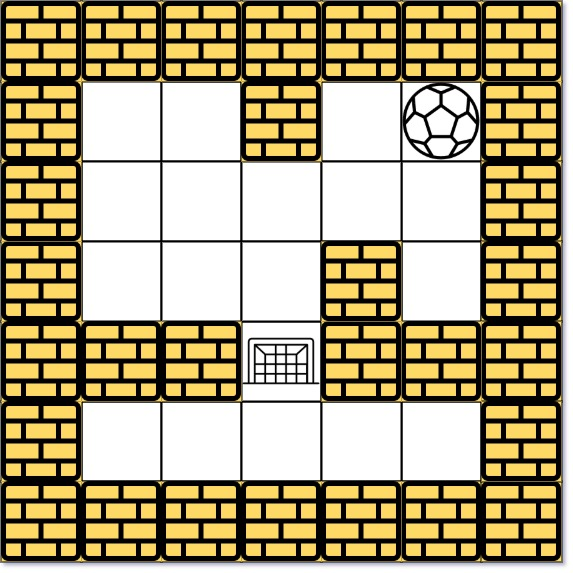
\includegraphics[width=0.25\linewidth]{images/lc0490_eg2}
\label{fig:lc0490eg2}
\end{figure}
Notice that you can pass through the destination but you cannot stop there.
\end{itemize}

\subsection*{Solution - DFS}
\begin{lstlisting}

bool hasPath(std::vector<std::vector<int>>& maze, std::vector<int>& start,
             std::vector<int>& destination) {
  std::vector<std::vector<bool>> visited(maze.size(),
                                         std::vector<bool>(maze[0].size(), false));
  return dfs(maze, start[0], start[1], destination, visited);
}

bool dfs(std::vector<std::vector<int>>& maze, int row, int col,
         std::vector<int>& destination, std::vector<std::vector<bool>>& visited) {
  // If we're out of bounds or at a wall, or if we've visited this point before, stop
  // exploring.
  if (!isValid(maze, row, col) || visited[row][col]) { return false; }

  // If we've reached the destination, return true.
  if (row == destination[0] && col == destination[1]) { return true; }

  // Mark this point as visited.
  visited[row][col] = true;

  // Roll the ball in each direction until it hits a wall.
  int i, j;
  // Up
  for (i = row; isValid(maze, i - 1, col); --i)
    ;
  if (dfs(maze, i, col, destination, visited)) return true;

  // Down
  for (i = row; isValid(maze, i + 1, col); ++i)
    ;
  if (dfs(maze, i, col, destination, visited)) return true;

  // Left
  for (j = col; isValid(maze, row, j - 1); --j)
    ;
  if (dfs(maze, row, j, destination, visited)) return true;

  // Right
  for (j = col; isValid(maze, row, j + 1); ++j)
    ;
  if (dfs(maze, row, j, destination, visited)) return true;

  // If none of the paths worked out, return false.
  return false;
}

// Helper function to check if a position is within the bounds and not a wall.
bool isValid(std::vector<std::vector<int>>& maze, int row, int col) {
  return row >= 0 && col >= 0 && row < maze.size() && col < maze[0].size()
         && maze[row][col] == 0;
}
\end{lstlisting}

\section{LC 0934 - Shortest Bridge}
You are given an {\colorbox{CodeBackground}{\lstinline|n x n|}} binary matrix {\colorbox{CodeBackground}{\lstinline|grid|}} where {\colorbox{CodeBackground}{\lstinline|1|}} represents \ul{land} and {\colorbox{CodeBackground}{\lstinline|0|}} represents \ul{water}.\\

An \ul{island} is a {\colorbox{CodeBackground}{\lstinline|4|}}-directionally connected group of {\colorbox{CodeBackground}{\lstinline|1|}}'s not connected to any other {\colorbox{CodeBackground}{\lstinline|1|}}'s. \\

There are \ul{exactly two islands} in {\colorbox{CodeBackground}{\lstinline|grid|}}.\\

You may change {\colorbox{CodeBackground}{\lstinline|0|}}'s to {\colorbox{CodeBackground}{\lstinline|1|}}'s to connect the two islands to form one island.\\

Return the smallest number of {\colorbox{CodeBackground}{\lstinline|0|}}'s you must flip to connect the two islands.\\

\begin{itemize}
	\item Example 1
\begin{lstlisting}
[[0,1],
 [1,0]] --> 1
\end{lstlisting}
	\item Example 2
\begin{lstlisting}
[[0,1,0],
 [0,0,0],
 [0,0,1]] --> 2
\end{lstlisting}
	\item Example 3
\begin{lstlisting}
[[1,1,1,1,1],
 [1,0,0,0,1],
 [1,0,1,0,1],
 [1,0,0,0,1],
 [1,1,1,1,1]]--> 1
\end{lstlisting}
\end{itemize}

\subsection*{Solution - DFS + BFS}
\begin{lstlisting}
int shortestBridge(std::vector<std::vector<int>>& grid) {
  // find and mark the first island (grid[i][j] == 2)
  std::queue<std::pair<int, int>> q;
  bool found = false;
  for (int i = 0; i < grid.size(); ++i) {
    if (found) { break; }
    for (int j = 0; j < grid[0].size(); ++j) {
      if (grid[i][j] == 1) {
        DFSMarkFirstIsland(grid, i, j, q);
        found = true;
        break;
      }
    }
  }
  // expand the first island until we reach the second one
  int num_step = 0;
  std::vector<std::pair<int, int>> dirs = {{-1, 0}, {1, 0}, {0, -1}, {0, 1}};
  while (!q.empty()) {
    int level_size = q.size();
    for (int i = 0; i < level_size; ++i) {
      auto [r, c] = q.front();
      q.pop();
      for (auto [dr, dc] : dirs) {
        int new_r = r + dr;
        int new_c = c + dc;
        if (new_r >= 0 && new_c >= 0 && new_r < grid.size() && new_c < grid[0].size()
            && grid[new_r][new_c] != 2) {
          if (grid[new_r][new_c] == 1) { return num_step; }
          q.emplace(new_r, new_c);
          grid[new_r][new_c] = 2;
        }
      }
    }
    ++num_step;
  }
  return -1;
}

void DFSMarkFirstIsland(std::vector<std::vector<int>>& grid, int r, int c,
                        std::queue<std::pair<int, int>>& q) {
  if (r < 0 || c < 0 || r >= grid.size() || c >= grid[0].size()) { return; }
  if (grid[r][c] != 1) { return; }
  grid[r][c] = 2;
  q.emplace(r, c);
  DFSMarkFirstIsland(grid, r - 1, c, q);
  DFSMarkFirstIsland(grid, r + 1, c, q);
  DFSMarkFirstIsland(grid, r, c - 1, q);
  DFSMarkFirstIsland(grid, r, c + 1, q);
}
\end{lstlisting}

\section{LC 0542 - 01 Matrix}
Given an {\colorbox{CodeBackground}{\lstinline|m x n|}} binary matrix {\colorbox{CodeBackground}{\lstinline|mat|}}, return the distance of the nearest {\colorbox{CodeBackground}{\lstinline|0|}} for each cell.

\begin{itemize}
\item Example 1
\begin{lstlisting}
[[0,0,0],
 [0,1,0],
 [0,0,0]]
-->
[[0,0,0],
 [0,1,0],
 [0,0,0]]
\end{lstlisting}
\item Example 2
\begin{lstlisting}
[[0,0,0],
 [0,1,0],
 [1,1,1]]
-->
[[0,0,0],
 [0,1,0],
 [1,2,1]]
\end{lstlisting}
\end{itemize}

\subsection*{Solution - BFS + DP}
\begin{lstlisting}
std::vector<std::vector<int>> updateMatrix(std::vector<std::vector<int>>& mat) {
  int m = mat.size();
  int n = mat[0].size();
  std::vector<std::vector<int>> dist(m,
                                     std::vector<int>(n, std::numeric_limits<int>::max()));
  std::queue<std::pair<int, int>> q;
  for (int i = 0; i < m; ++i) {
    for (int j = 0; j < n; ++j) {
      if (mat[i][j] == 0) {
        dist[i][j] = 0;
        q.emplace(i, j);
      }
    }
  }
  std::vector<std::pair<int, int>> dirs = {{-1, 0}, {1, 0}, {0, -1}, {0, 1}};
  while (!q.empty()) {
    auto [r, c] = q.front();
    q.pop();
    for (auto [dr, dc] : dirs) {
      int new_r = r + dr;
      int new_c = c + dc;
      if (new_r >= 0 && new_r < m && new_c >= 0 && new_c < n) {
        if (dist[new_r][new_c] > dist[r][c] + 1) {
          dist[new_r][new_c] = dist[r][c] + 1;
          q.emplace(new_r, new_c);
        }
      }
    }
  }
  return dist;
}
\end{lstlisting}

\section{LC 2812 - Find the Safest Path in a Grid}
You are given a {\colorbox{CodeBackground}{\lstinline|0|}}-indexed 2D matrix {\colorbox{CodeBackground}{\lstinline|grid|}} of size {\colorbox{CodeBackground}{\lstinline|n x n|}}, where {\colorbox{CodeBackground}{\lstinline|(r, c)|}} represents:
\begin{itemize}
\item A cell containing a thief, if {\colorbox{CodeBackground}{\lstinline|grid[r][c] = 1|}}.
\item An empty cell, if {\colorbox{CodeBackground}{\lstinline|grid[r][c] = 0|}}.
\end{itemize}

You are initially positioned at cell {\colorbox{CodeBackground}{\lstinline|(0, 0)|}} and you want to move to {\colorbox{CodeBackground}{\lstinline|(n - 1, n - 1)|}}. In one move, you can move to any \ul{adjacent cell} ({\colorbox{CodeBackground}{\lstinline|4|}}-directionally) in the grid, including cells containing thieves. The \ul{safeness factor} of a \ul{path} is defined as the \ul{minimum Manhattan distance} from \ul{any cell in the path} to \ul{any thief in the grid}. Return the \ul{maximum safeness factor} of all paths from cell {\colorbox{CodeBackground}{\lstinline|(0, 0)|}} to cell {\colorbox{CodeBackground}{\lstinline|(n - 1, n - 1)|}}. \\

The \ul{Manhattan distance} between two cells {\colorbox{CodeBackground}{\lstinline|(x_1, y_1)|}} and {\colorbox{CodeBackground}{\lstinline|(x_2, y_2)|}} is equal to {\colorbox{CodeBackground}{\lstinline|\|x_1 - x_2\| + \|y_1 - y_2\||}}. 

\begin{itemize}
\item Example 1
\begin{lstlisting}
[[1,0,0],
 [0,0,0],
 [0,0,1]] --> 0
\end{lstlisting}
\begin{figure}[H]
\centering
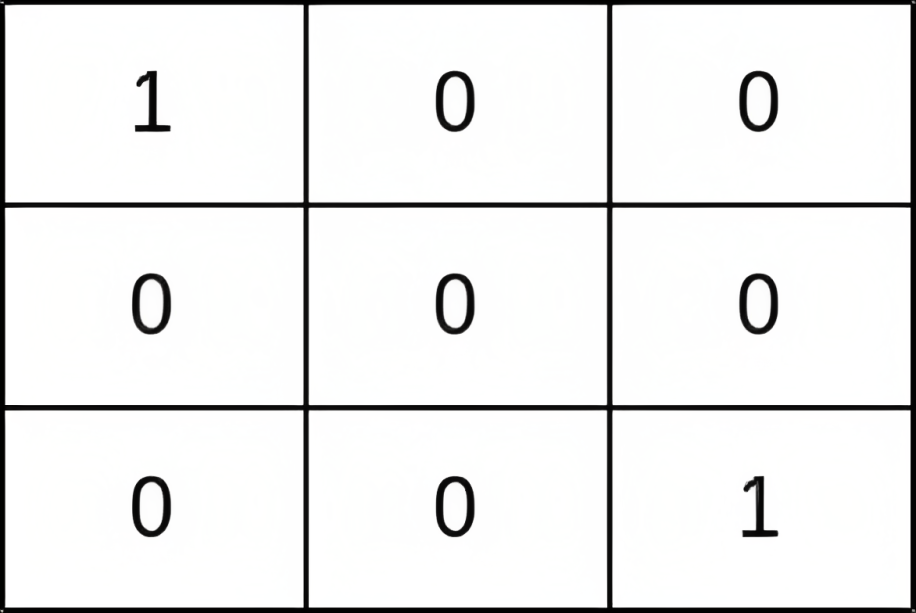
\includegraphics[width=0.2\linewidth]{images/lc2812_eg1}
\label{fig:lc2812eg1}
\end{figure}
All paths from {\colorbox{CodeBackground}{\lstinline|(0, 0)|}} to {\colorbox{CodeBackground}{\lstinline|(n - 1, n - 1)|}} go through the thieves in cells {\colorbox{CodeBackground}{\lstinline|(0, 0|}}) and {\colorbox{CodeBackground}{\lstinline|(n - 1, n - 1)|}}.
	\item Example 2
\begin{lstlisting}
[[0,0,1],
 [0,0,0],
 [0,0,0]] --> 2
\end{lstlisting}
\begin{figure}[H]
\centering
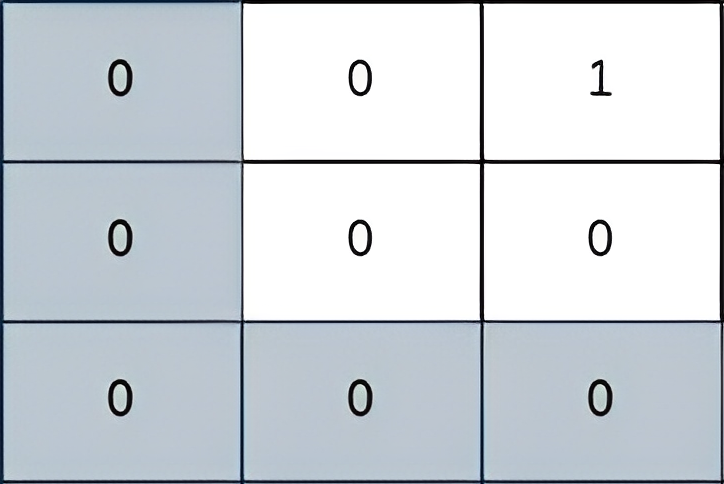
\includegraphics[width=0.2\linewidth]{images/lc2812_eg2}
\label{fig:lc2812eg2}
\end{figure}
\item Example 3
\begin{lstlisting}
[[0,0,0,1],
 [0,0,0,0],
 [0,0,0,0],
 [1,0,0,0]] --> 2
\end{lstlisting}
\begin{figure}[H]
\centering
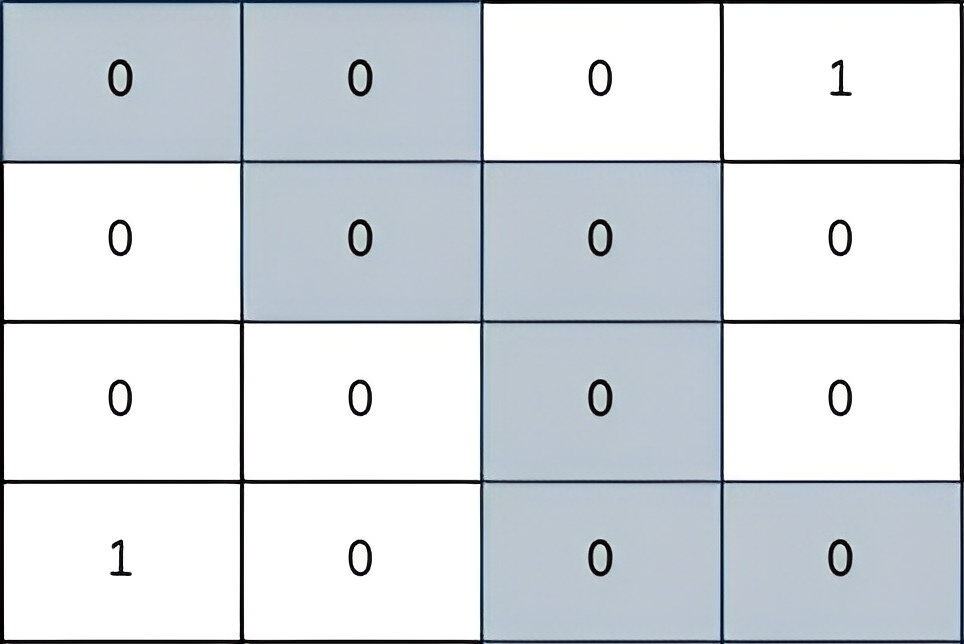
\includegraphics[width=0.26\linewidth]{images/lc2812_eg3}
\label{fig:lc2812eg3}
\end{figure}
\end{itemize}

\section{LC 0304 - Range Sum Query 2D - Immutable}\label{lc0304}
\hyperref[sec:prefix_sum]{[Prefix Sum]}\\

Given a \ul{non-empty} 2D matrix {\colorbox{CodeBackground}{\lstinline|matrix|}}, handle multiple queries of the following type:\\

Calculate the sum of the elements of {\colorbox{CodeBackground}{\lstinline|matrix|}} inside the rectangle defined by its upper left corner {\colorbox{CodeBackground}{\lstinline|(row1, col1)|}} and lower right corner {\colorbox{CodeBackground}{\lstinline|(row2, col2)|}}.\\

Implement the {\colorbox{CodeBackground}{\lstinline|NumMatrix|}} class:
\begin{itemize}
\item {\colorbox{CodeBackground}{\lstinline|NumMatrix(int[][] matrix)|}} - Initializes the object with the integer matrix {\colorbox{CodeBackground}{\lstinline|matrix|}}.
\item {\colorbox{CodeBackground}{\lstinline|int sumRegion(int row1, int col1, int row2, int col2)|}} - Returns the sum of the elements of {\colorbox{CodeBackground}{\lstinline|matrix|}} inside the rectangle defined by its upper left corner {\colorbox{CodeBackground}{\lstinline|(row1, col1)|}} and lower right corner {\colorbox{CodeBackground}{\lstinline|(row2, col2)|}}.
\end{itemize}

\subsection*{Solution 1 - Prefix Sum (size $(m + 1) \times (n + 1))$}
\begin{lstlisting}
class NumMatrix {
 public:
  NumMatrix(std::vector<std::vector<int>>& matrix) {
    int m = matrix.size();
    int n = matrix[0].size();
    prefix_sum_ = std::vector<std::vector<int>>(m + 1, std::vector<int>(n + 1, 0));
    for (int i = 0; i < m; ++i) {
      for (int j = 0; j < n; ++j) {
        prefix_sum_[i + 1][j + 1] =
            matrix[i][j] + prefix_sum_[i][j + 1] + prefix_sum_[i + 1][j] - prefix_sum_[i][j];
      }
    }
  }

  int sumRegion(int row1, int col1, int row2, int col2) {
    return prefix_sum_[row2 + 1][col2 + 1] - prefix_sum_[row2 + 1][col1]
           - prefix_sum_[row1][col2 + 1] + prefix_sum_[row1][col1];
  }

 private:
  std::vector<std::vector<int>> prefix_sum_;
};
\end{lstlisting}

\subsection*{Solution 2 - Prefix Sum (size $m \times n$)}
\begin{lstlisting}
class NumMatrix {
 public:
  NumMatrix(std::vector<std::vector<int>>& matrix) {
    int m = matrix.size();
    int n = matrix[0].size();
    prefix_sum_ = std::vector<std::vector<int>>(m, std::vector<int>(n, 0));
    for (int i = 0; i < m; ++i) {
      for (int j = 0; j < n; ++j) {
        prefix_sum_[i][j] = matrix[i][j] + (i == 0 ? 0 : prefix_sum_[i - 1][j])
                            + (j == 0 ? 0 : prefix_sum_[i][j - 1])
                            - (i == 0 || j == 0 ? 0 : prefix_sum_[i - 1][j - 1]);
      }
    }
  }

  int sumRegion(int row1, int col1, int row2, int col2) {
    return prefix_sum_[row2][col2] - (row1 == 0 ? 0 : prefix_sum_[row1 - 1][col2])
           - (col1 == 0 ? 0 : prefix_sum_[row2][col1 - 1])
           + (row1 == 0 || col1 == 0 ? 0 : prefix_sum_[row1 - 1][col1 - 1]);
  }

 private:
  std::vector<std::vector<int>> prefix_sum_;
};
\end{lstlisting}

\subsection*{Related}
\begin{itemize}
\item \hyperref[lc0303]{LC 0303 - Range Sum Query - Immutable}
\item \hyperref[lc0304]{LC 0304 - Range Sum Query 2D - Immutable}
\end{itemize}

\section{LC 2017 - Grid Game}\label{lc2017}
\hyperref[sec:prefix_sum]{[Prefix Sum]}\\

You are given a {\colorbox{CodeBackground}{\lstinline|0|}}-indexed 2D array {\colorbox{CodeBackground}{\lstinline|grid|}} of size {\colorbox{CodeBackground}{\lstinline|2 x n|}} ({\colorbox{CodeBackground}{\lstinline|n >= 1|}}), where {\colorbox{CodeBackground}{\lstinline|grid[r][c] >= 1|}} represents the number of points at position {\colorbox{CodeBackground}{\lstinline|(r, c)|}} on the matrix. Two robots are playing a game on this matrix.\\

Both robots initially start at {\colorbox{CodeBackground}{\lstinline|(0, 0)|}} and want to reach {\colorbox{CodeBackground}{\lstinline|(1, n - 1)|}}. \\

Each robot may only move to the right {\colorbox{CodeBackground}{\lstinline|((r, c) to (r, c + 1))|}} or down {\colorbox{CodeBackground}{\lstinline|((r, c) to (r + 1, c))|}}.\\

At the start of the game, the first robot moves from {\colorbox{CodeBackground}{\lstinline|(0, 0)|}} to {\colorbox{CodeBackground}{\lstinline|(1, n - 1)|}}, collecting all the points from the cells on its path. For all cells {\colorbox{CodeBackground}{\lstinline|(r, c)|}} traversed on the path, {\colorbox{CodeBackground}{\lstinline|grid[r][c]|}} is set to {\colorbox{CodeBackground}{\lstinline|0|}}. Then, the second robot moves from {\colorbox{CodeBackground}{\lstinline|(0, 0)|}} to {\colorbox{CodeBackground}{\lstinline|(1, n-1)|}}, collecting the points on its path. Note that their paths may intersect with one another.\\

The first robot wants to minimize the number of points collected by the second robot. In contrast, the second robot wants to maximize the number of points it collects. If both robots play optimally, return the number of points collected by the second robot.

\begin{itemize}
\item {\colorbox{CodeBackground}{\lstinline|grid = [[2,5,4],[1,5,1]] --> 4|}}
\begin{figure}[H]
\centering
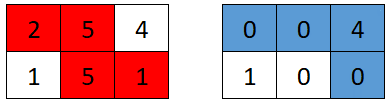
\includegraphics[width=0.3\linewidth]{images/lc2017_eg1}
\end{figure}
The optimal path taken by the first robot is shown in red, and the optimal path taken by the second robot is shown in blue.\\
The cells visited by the first robot are set to {\colorbox{CodeBackground}{\lstinline|0|}}.\\
The second robot will collect {\colorbox{CodeBackground}{\lstinline|0 + 0 + 4 + 0 = 4|}} points.
\item {\colorbox{CodeBackground}{\lstinline|grid = [[3,3,1],[8,5,2]] --> 4|}}
\begin{figure}[H]
\centering
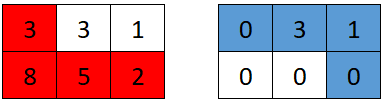
\includegraphics[width=0.3\linewidth]{images/lc2017_eg2}
\end{figure}
The optimal path taken by the first robot is shown in red, and the optimal path taken by the second robot is shown in blue.\\
The cells visited by the first robot are set to {\colorbox{CodeBackground}{\lstinline|0|}}.\\
The second robot will collect {\colorbox{CodeBackground}{\lstinline|0 + 3 + 1 + 0 = 4|}} points.
\item {\colorbox{CodeBackground}{\lstinline|grid = [[1,3,1,15],[1,3,3,1]] --> 7|}}
\begin{figure}[H]
\centering
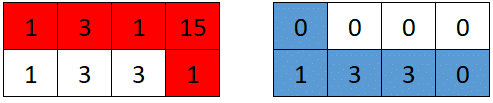
\includegraphics[width=0.38\linewidth]{images/lc2017_eg3}
\end{figure}
The optimal path taken by the first robot is shown in red, and the optimal path taken by the second robot is shown in blue.\\
The cells visited by the first robot are set to {\colorbox{CodeBackground}{\lstinline|0|}}.\\
The second robot will collect {\colorbox{CodeBackground}{\lstinline|0 + 1 + 3 + 3 + 0 = 7|}} points.
\end{itemize}

\subsection*{Solution - Prefix Sum {\scriptsize\color{gray}\Coffeecup\hspace{1mm}Time $O(n)$, Space $O(n)$}}
\begin{lstlisting}
long long gridGame(std::vector<std::vector<int>>& grid) {
  int n = grid[0].size();
  std::vector<long> top_prefix_sum(n + 1, 0);
  std::vector<long> bottom_prefix_sum(n + 1, 0);
  for (int i = 1; i <= n; ++i) {
    top_prefix_sum[i] = grid[0][i - 1] + top_prefix_sum[i - 1];
    bottom_prefix_sum[i] = grid[1][i - 1] + bottom_prefix_sum[i - 1];
  }
  long long max_second_robot = LLONG_MAX;
  for (int i = 0; i < n; ++i) {
    long long top_sum = top_prefix_sum[n] - top_prefix_sum[i + 1];
    long long bottom_sum = bottom_prefix_sum[i];
    max_second_robot = std::min(max_second_robot, std::max(top_sum, bottom_sum));
  }
  return max_second_robot;
}
\end{lstlisting}

\subsection*{Solution - Prefix Sum, Optimized {\scriptsize\color{gray}\Coffeecup\hspace{1mm}Time $O(n)$, Space $O(1)$}}
\begin{lstlisting}
long long gridGame(std::vector<std::vector<int>>& grid) {
  long long top_sum = std::accumulate(grid[0].begin(), grid[0].end(), 0LL);
  long long bottom_sum = 0;
  long long max_second_robot = LLONG_MAX;
  for (int i = 0; i < grid[0].size(); ++i) {
    top_sum -= grid[0][i];
    max_second_robot = std::min(max_second_robot, std::max(top_sum, bottom_sum));
    bottom_sum += grid[1][i];
  }
  return max_second_robot;
}
\end{lstlisting}

\section{LC 0329 - Longest Increasing Path in a Matrix}
Given an {\colorbox{CodeBackground}{\lstinline|m x n|}} integers {\colorbox{CodeBackground}{\lstinline|matrix|}}, return the length of the longest increasing path in {\colorbox{CodeBackground}{\lstinline|matrix|}}.\\

From each cell, you can either move in four directions: \ul{left}, \ul{right}, \ul{up}, or \ul{down}. You may not move diagonally or move outside the boundary (i.e., wrap-around is not allowed).\\

\begin{itemize}
\item Example 1: {\colorbox{CodeBackground}{\lstinline|matrix = [[9,9,4],[6,6,8],[2,1,1]] --> 4|}}
\begin{figure}[H]
\centering
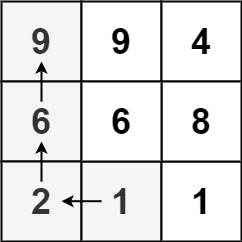
\includegraphics[width=0.15\linewidth]{images/lc0329_eg1}
\label{fig:lc0329eg1}
\end{figure}
\item Example 2: {\colorbox{CodeBackground}{\lstinline|matrix = [[3,4,5],[3,2,6],[2,2,1]] --> 4|}}
\begin{figure}[H]
\centering
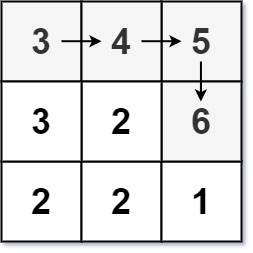
\includegraphics[width=0.15\linewidth]{images/lc0329_eg2}
\label{fig:lc0329eg2}
\end{figure}
\item {\colorbox{CodeBackground}{\lstinline|matrix = [[1]] --> 1|}}
\end{itemize}

\subsection*{Solution - DFS}
\begin{lstlisting}
// Utility function to perform DFS and memoization
int dfs(const std::vector<std::vector<int>>& matrix, int i, int j,
        std::vector<std::vector<int>>& memo) {
  // If we already know the longest path from this cell, return it
  if (memo[i][j] != 0) { return memo[i][j]; }

  // Directions in which we can move: up, down, left, right
  std::vector<std::pair<int, int>> dirs = {{-1, 0}, {1, 0}, {0, -1}, {0, 1}};
  // Initialize the length of the longest path from this cell
  int max_path = 1;

  // Explore all the possible directions
  for (const auto& dir : dirs) {
    int x = i + dir.first, y = j + dir.second;

    // Check if the new position is within bounds and the value is greater than the current
    // cell
    if (x >= 0 && y >= 0 && x < matrix.size() && y < matrix[0].size()
        && matrix[x][y] > matrix[i][j]) {
      // DFS from the new position
      int len = 1 + dfs(matrix, x, y, memo);
      // Update the longest path from the current cell
      max_path = std::max(max_path, len);
    }
  }

  // Memoize the result
  memo[i][j] = max_path;
  return max_path;
}

int longestIncreasingPath(std::vector<std::vector<int>>& matrix) {
  int m = matrix.size();
  int n = matrix[0].size();
  std::vector<std::vector<int>> memo(m, std::vector<int>(n, 0));
  int longest_path = 0;
  for (int i = 0; i < m; ++i) {
    for (int j = 0; j < n; ++j) {
      longest_path = std::max(longest_path, dfs(matrix, i, j, memo));
    }
  }
  return longest_path;
}
\end{lstlisting}

\section{LC 0048 - Rotate Image}
You are given an {\colorbox{CodeBackground}{\lstinline|n x n|}} 2D {\colorbox{CodeBackground}{\lstinline|matrix|}} representing an image, rotate the image by 90 degrees (clockwise).\\

You have to rotate the image \ul{in-place}, which means you have to modify the input 2D matrix directly.

\begin{itemize}
\item Example 1:
\begin{figure}[H]
\centering
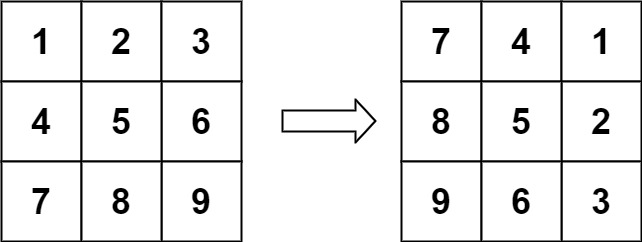
\includegraphics[width=0.4\linewidth]{images/lc0048_eg1}
\end{figure}
\item Example 2:
\begin{figure}[H]
\centering
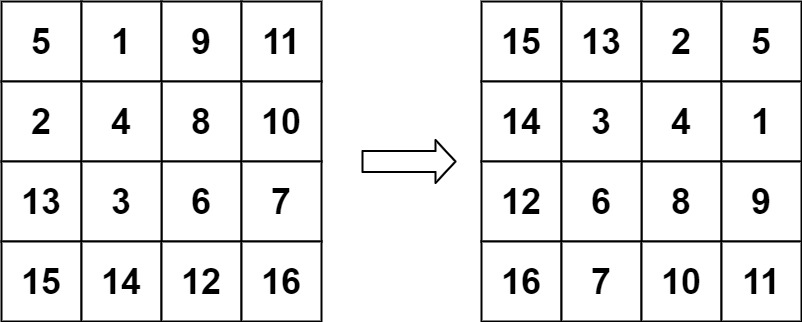
\includegraphics[width=0.5\linewidth]{images/lc0048_eg2}
\end{figure}
\end{itemize}

\subsection*{Solution 1 - Brute Force}
\begin{lstlisting}
void rotate(std::vector<std::vector<int>>& matrix) {
  int n = matrix.size();
  for (int layer = 0; layer < n / 2; ++layer) {
    int first = layer;
    int last = n - 1 - layer;
    for (int i = first; i < last; ++i) {
      int offset = i - first;
      int top = matrix[first][i];  // save top
      // left -> top
      matrix[first][i] = matrix[last - offset][first];
      // bottom -> left
      matrix[last - offset][first] = matrix[last][last - offset];
      // right -> bottom
      matrix[last][last - offset] = matrix[i][last];
      // top -> right
      matrix[i][last] = top;  // right <- saved top
    }
  }
}
\end{lstlisting}

\subsection*{Solution 2 - Transpose and Reverse}
\begin{lstlisting}
void rotate(std::vector<std::vector<int>>& matrix) {
  // transpose the matrix
  for (int i = 0; i < matrix.size(); ++i) {
    for (int j = i; j < matrix.size(); ++j) { std::swap(matrix[i][j], matrix[j][i]); }
  }
  // reverse each row
  for (auto& row : matrix) { std::reverse(row.begin(), row.end()); }
}
\end{lstlisting}